\chapter{Third Species of Counterpoint}

The third species of counterpoint consists of four notes by measure, four notes against one note. In other words, only quarter notes.
\begin{figure}[h]
    \centering
    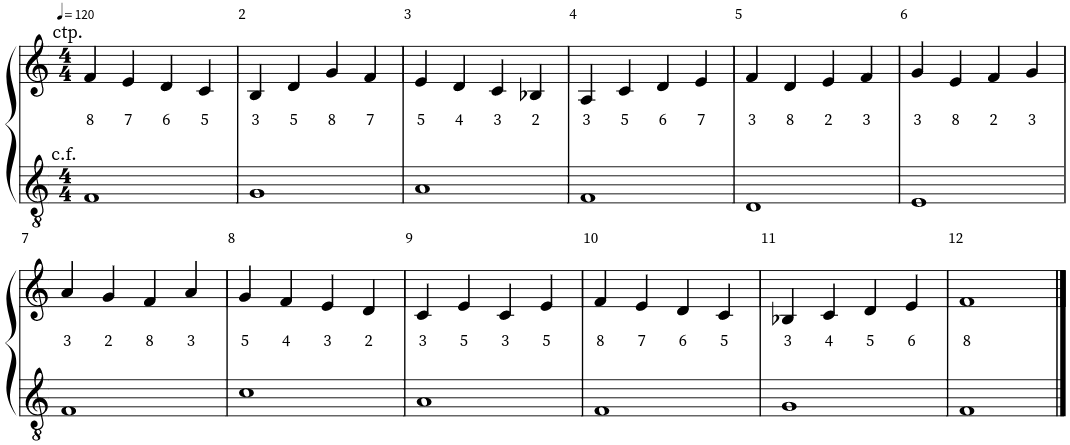
\includegraphics[width=5in]{Images/complete_third_species_f.png}
    \caption{Example of a \species{3} ctp. \listen{Listen3SP} \listenyt{https://youtu.be/9yB4OGr4Cgk?t=127}}
\end{figure}

As in the previous chapter, the rules of the first species are applied to the thesis note, i.e. the first note of the group of four quarter notes. The first note of a measure is always the most important\footnote{Unless there is syncopation as it will be explained in the next chapter.}, it is the one that establishes the main harmony perceived by the human ear. To sum up, first species harmonic rules are applied in thesis, while first species melodic rules are applied for all notes, and first species motions rules are adapted to the species.

The third species is the one that starts to be vague in the explanations given by Fux. Admittedly, he probably didn't expect his work to be formalized through constraint programming. But even for musicians, there's no denying that some rules lack illustrative examples and are a bit skimmed over. In addition, the original treatise is in Latin and, despite access to several translations in French and English, the explanations do not always mean exactly the same thing, and everyone knows that the devil's in the details. This is reflected, for example, in the formalization of the first two harmonic rules, which are both created from fuzzy explanations and different translations.

\section{Formalization in English}

% \paragraph{}\textbf{Harmonic} rules of the third species are the following:
\subsection{Harmonic rules of the third species}
\begin{enumerate}[wide, label=\bfseries 3.H\arabic*]
    \item\label{rule:fivequarters} \textit{If five notes follow each other by joint degrees in the same direction, then the harmonic interval of the third note must be consonant.} \textcite[p.73]{GaPFr}

    The following analysis is more the work of a historian than a computer scientist. The resulting formalization is therefore not the only way to go. As explained above, not all translations are equivalent. \citeauthor{GaPFr}'s French translation, which is the most recent and used as the main source in this thesis, says (see the original text in the appendix at \ref{appen:cinqnoires}):
    % Which can be literally translated as:
    \begin{quote}
        If it happens that five quarter notes follow each other \textbf{by joint degrees}, either ascending or descending, the first one must be consonant, the second one may be dissonant, the third one again necessarily consonant, the fourth one may be dissonant \textbf{if} the fifth one is a consonance.
    \end{quote}

    In contrast, \citeauthor{GaPEng}'s English translation says:
    \begin{quotation}
        "[\dots] if fives quarters follow each other either ascending or descending, the first one [\dots].
        % has to be consonant, the second one may be dissonant, and the third must again be consonant.
        The fourth one may be dissonant \textbf{if} the fifth is consonant [\dots]."
        \textcite[p.50]{GaPEng}
    \end{quotation}

    Alternatively, other older references as \parencite[p.51]{IMSLPfr} and \parencite[p.4]{IMSLPeng} from the XVIII century basically say:
    \begin{quote}
        When five quarters follow one another \textbf{gradually} either rising or falling, the first, third \textbf{and} fifth note \textbf{must} be consonant. While the second and fourth may be dissonant.
    \end{quote}

    Several issues arise from these previous sentences. First, \citeauthor{GaPEng}'s English version does not say "gradually" or "by joint degree" which changes the rule itself. These terms make the constraint much more precise and therefore less restrictive. It can be said without too much hesitation that the rule must be applied only in the case of joint degrees because most translations propose a "gradually"\footnote{In the original Latin text, \textcite[p.63]{IMSLPlatin} states "continuò gradatim", which can be translated by "step by step".}. Moreover, Fux's examples confirm this hypothesis.

    Second problem: "\textbf{if} the fifth note is consonant". Why "if"? Actually, it's more complicated than that. For this rule, Fux does not explain if he is talking about:
    \begin{enumerate}
        \item the four quarter notes of a measure plus the first one of the next measure;
        \item any five-note tuple;
        \item any independent five-note tuple that doesn't overlap with the previous one.
    \end{enumerate}
    
    In Fux's examples, more than five notes follow each other several times, up to nine notes in a row in some. If the second assumption were true, then the following figure \ref{fig:nineiar} from the book would not be correct.
    \begin{figure}[h]
        \centering
        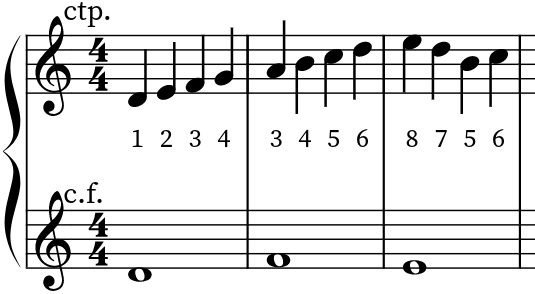
\includegraphics[height=\fh]{Images/nine_quarters.png}
        \caption{Nine quarters that follow each other gradually, \species{3}.}
        \label{fig:nineiar}
    \end{figure}

    The third hypothesis (c) that states that Fux talks of \emph{any five-note tuple as long as it is not itself in a previous five-note tuple} does not work either. Otherwise, figure \ref{fig:sixiar} would not be right.
    \begin{figure}[h]
        \centering
        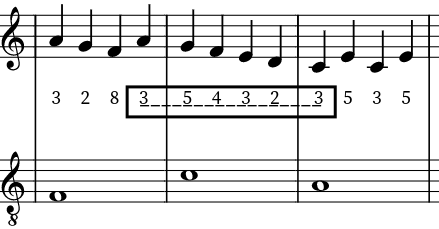
\includegraphics[height=\fh]{Images/six_quarters.png}
        \caption{Six quarters that follow each other gradually where the \nth{3} one is dissonant, \species{3}.}
        \label{fig:sixiar}
    \end{figure}

    It is clear that the third note is dissonant whereas with assumption (a), the rule would be maintained. As a result, it was decided that the first hypothesis was the right one. But it does not explain why it is said "if the fifth note is consonant". With this hypothesis, the fifth note is a thesis note and is therefore necessarily consonant thanks to rule \ref{rule:consthesis}. In the end, since saying that a note "may be dissonant" actually means that no constraint is added, the only additional constraint is the one on the third note.

    \item\label{rule:thirddiss} \textit{If the third harmonic interval of a measure is dissonant then the second and the fourth interval must be consonant and the third note must be a diminution\footnote{An intermediate note that fills a skip of third.}.} \parencite[p.73-74]{GaPFr}

    Stepping back, this rule can be \emph{partly} written in another more meaningful way: \textit{any dissonance implies that it is surrounded by consonances}. Which makes sense in music because, in a melody, dissonances are often used to link the consonant notes of an explicit or implicit chord. The logical proof is given in the mathematical section \ref{sec:math3sp} that follows.

    \item\label{rule:cambiata} \textit{It is best to avoid the second and third harmonies of a measure to be consonant with a one-degree melodic interval between them.} \parencite[p.74-75]{GaPFr}
    
    Fux calls this rule the \textit{cambiata} note\footnote{Literally translated from Italian to the "\emph{exchanged} note". \parencite[p.51]{GaPEng}}. This rule is followed by composers of authority who stimulate the use of dissonances. As shown in figure \ref{fig:cambiata}, the seventh interval of the second note should be played rather than the sixth.
    \begin{figure}[h]
        \centering
        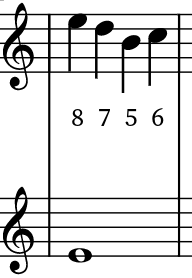
\includegraphics[height=\fh]{Images/cambiata.png}
        \caption{Use of the \textit{cambiata} note in the second quarter.}
        \label{fig:cambiata}
    \end{figure}
    
    \item\label{rule:penult3sp} \textit{In addition to rule \ref{rule:up_penult}, in the penultimate measure, if the \cf is in the upper part, then the harmonic interval of the first note should be a minor third.} \parencite[p.75]{GaPFr}

    Fux, for some reason, does not always follow this rule, which he gives in a very crude way with a single example (figure \ref{fig:penult3sp}) to follow without further explanation. % "If the \cf occurs in the upper part, the possibilities are these:" \textcite[p.52]{GaPEng}.
    The only particularity of this measure is in the first and last note which are minor thirds, which is consistent.

    \begin{figure}[h]
        \centering
        \begin{subfigure}{.5\textwidth}
            \centering
            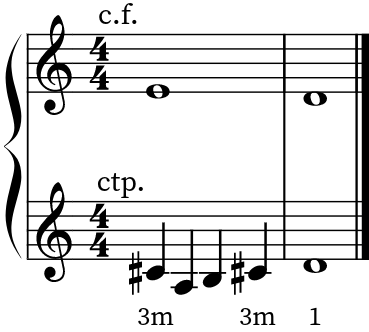
\includegraphics[height=\fh]{Images/penult_3rd.png}
            \caption{Standard penultimate measure.}
            \label{fig:penult3sp}
        \end{subfigure}%
        \begin{subfigure}{.5\textwidth}
            \centering
            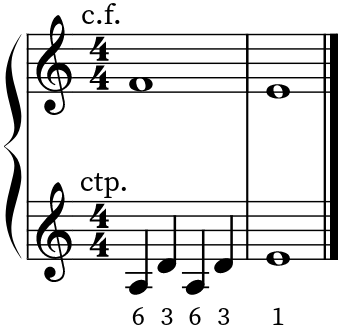
\includegraphics[height=\fh]{Images/penult_deviation_3rd.png}
            \caption{Fux's deviation.}
            \label{fig:penultdeviation}
        \end{subfigure}
        \caption{Different penultimate measures, \species{3}.}
    \end{figure}

    However, Fux gives this example (figure \ref{fig:penultdeviation}) which is not detailed. Luckily, \citeauthor{GaPEng} has footnoted that:
    \begin{quotation}
        "The forming of sequences (the so-called monotonia) ought to be avoided as far as possible. In the original [a] correction for the next to the last measure was added in manuscript".
        \textcite[p.54]{GaPEng}
    \end{quotation}

    This correction is yet another way of writing the penultimate measure. There is nothing wrong with Fux allowing deviations, that is what music is about in a way. But it makes systematic formalization more difficult. It was chosen to ignore this example and leave this rule optional because of its inconsistency with the rest.
\end{enumerate}

\subsection{Melodic rules of the third species}
The melodic rule \ref{rule:notsamecons} of the second species is applied to all notes.

\begin{enumerate}[wide, label=\bfseries 3.M\arabic*]
    \item\label{rule:twobeats} \textit{Each note and its two beats further peer are preferred to be different.*\footnote{"*" means that this rule is implicit.}}
    
    This implicit rule is already generally present. It is kind of complementary to rule \ref{rule:notsamecons} but in a softer way. It happens several times in Fux's work that the pupil prefers to put himself in difficulty to avoid monotony in the melody. An important aspect of this monotony can be found in the repetition of notes. In this species, it becomes important because not taking that into account could lead to having only two different notes per measure (see figure \ref{fig:twonotes}), which could be considered "boring". The cost of this parameter is still adjustable by the user.
    \begin{figure}[h]
        \centering
        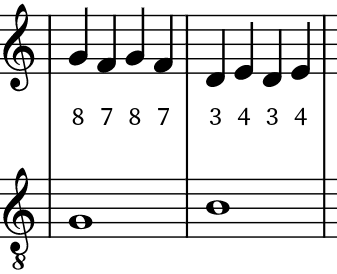
\includegraphics[height=\fh]{Images/two_same_notes.png}
        \caption{"Boring" example with only two different notes per measure, \species{3}.}
        \label{fig:twonotes}
    \end{figure}
\end{enumerate}

\subsection{Motion rules of the third species}
\begin{enumerate}[wide, label=\bfseries 3.P\arabic*]
    \item\label{rule:motion3rd} \textit{The motion is perceived based on the fourth note.*}
    
    Fux stops talking about motions explicitly from the chapter on the third species. But the legacy of the first species, the idea of reaching perfect consonances by contrary motion, remains present in all his examples.
    \begin{figure}[h]
        \centering
        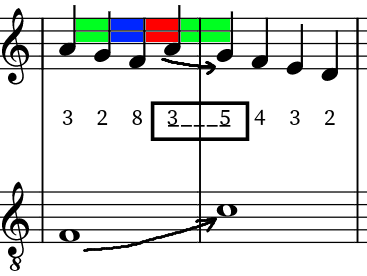
\includegraphics[height=\fh]{Images/motion_3rd.png}
        \caption{Contrary motion based on the fourth note. Colors represent that the motion is either \textcolor{green}{contrary}, \textcolor{blue}{oblique} or \textcolor{red}{direct}.}
        \label{fig:motion3rd}
    \end{figure}
    
    The motion is here (figure \ref{fig:motion3rd}) perceived from the note of the \cf with the fourth note of the counterpoint of the corresponding measure\footnote{Towards the next note of the \cf with the first note of the counterpoint of the corresponding measure.}. In fact, the third species allows more flexibility in the motions because with more notes it is possible to go up during the first three notes to come down (or vice versa) just before the start of the next measure to obtain the desired motion as seen in figure \ref{fig:motion3rd}.
\end{enumerate}

\section{Formalization into Constraints}\label{sec:math3sp}

\subsection{Harmonic Constraints of the Third Species}
\paragraph{\ref{rule:fivequarters}} \textit{If five notes follow each other by joint degrees in the same direction, then the harmonic interval of the third note must be consonant.}

\begin{equation}
    \begin{gathered}
        \forj\\
        % \{M[0, j]\land M[1, j]\land M[2, j]\land M[3, j]\} \leq 2\ \land\\
        % \left(
        %     \{M_{brut}[0, j]\land M_{brut}[1, j]\land M_{brut}[2, j]\land M_{brut}[3, j]\} > 0\ \lor \right. \\
        %     \left.
        %     \{M_{brut}[0, j]\land M_{brut}[1, j]\land M_{brut}[2, j]\land M_{brut}[3, j]\} < 0\
        % \right)\\
        % \implies IsCons[2, j]
        \left(
            \bigwedge_{i=0}^{3} M[i, j] \leq 2
        \right)
        \land
        \left(
            \bigwedge_{i=0}^{3} M_{brut}[i, j] > 0
            \lor
            \bigwedge_{i=0}^{3} M_{brut}[i, j] < 0
        \right)\\
        \implies IsCons[2, j]
    \end{gathered}
\end{equation}

On the one hand, the $M$ is used for the "joint degrees" property while the $M_{brut}$ for the "same direction" one.

\paragraph{\ref{rule:thirddiss}} \textit{If the third harmonic interval of a measure is dissonant then the second and the fourth interval must be consonant and the third note must be a diminution.}

To avoid negation in the code, which would require an additional step, the implication has been transformed into a logical or. The following constraints are set to be true.

\begin{equation}
    \begin{gathered}
        \forj\\
        IsCons[2, j] \lor \left( IsCons[1, j] \land IsCons[3, j] \land IsDim[j]\right)\\
        \text{where } IsDim[j]=\top \text{ when the \nth{3} note of the measure } j \text{ is a diminution.}
    \end{gathered}
\end{equation}

\paragraph{\ref{rule:cambiata}} \textit{It is best to avoid the second and third harmonies of a measure to be consonant with a one-degree melodic interval between them.}

The default value of $cost_{Cambiata}$ is \dfts{last resort} because Fux almost seems to forbid it but without a real musical reason to justify this convention.

\begin{equation}
    \begin{gathered}
        \forj\\
        Cambiata_{costs}[j] = \begin{cases}
            cost_{Cambiata} & \text{if } IsCons[1, j] \land IsCons[2, j] \land M[1, j] \leq 2\\
            0 & \text{otherwise}
        \end{cases}
    \end{gathered}
\end{equation}

\paragraph{\ref{rule:penult3sp}} \textit{In the penultimate measure, if the \cf is in the upper part, then the harmonic interval of the first note should be a minor third.}

\begin{equation}
    \begin{gathered}
        \lnot IsCfB[m-2] \implies H[0, m-2] = 3
    \end{gathered}
\end{equation}

\subsection{Melodic Constraints of the Third Species}
\paragraph{\ref{rule:twobeats}} \textit{Each note and its two beats further peer are preferred to be different.}

This rule is implicit so the default value of $cost_{MtwobSame}$ is \dfts{low cost}.

\begin{equation}
    \begin{gathered}
        \forpmm \\
        MtwoSame_{costs}[i, j] = \begin{cases}
            cost_{MtwobSame} & \text{if } M^2[\rho] = 0\\
            0 & \text{otherwise}
        \end{cases}
    \end{gathered}
\end{equation}

\subsection{Motion Constraints of the Third Species}
\paragraph{\ref{rule:motion3rd}} \textit{The motion is perceived based on the fourth note.}

This implies that the costs of the motions and the first species constraints on the motions are deducted from $P[3]$.